    本章ではまず、量子計算に用いられる一部の量子力学の公理について紹介する。
\section{量子ビット}
    \subsection{量子ビットの表現}
        古典コンピュータが電気信号のON,OFFを古典ビットの0,1に対応させるように、
        量子計算の基本単位を担う量子ビット(Quantum bit,略してQubitとも呼ばれる)は、ある量子系の固有状態をヒルベルト空間(内積を定義できるベクトル空間)$\mathcal{H}\in\mathbb{C}^2$上の
        \begin{equation}
            \ket{0}=\left(
                \begin{array}{c}
                  1\\
                  0\\
                \end{array}
              \right)
            ,
            \ket{1}=\left(
                \begin{array}{c}
                  0\\
                  1\\
                \end{array}
              \right)
        \end{equation}
        に対応させることで表現される。$\ket{0},\ket{1}$の元となる量子状態はスピンのアップ・ダウン、偏光の回転方向など様々にとることができるが
        本論文では後述する非線形調和振動子の光子数0個,1個の状態を$\ket{0}$,$\ket{1}$に対応させる。
        量子ビットの大きな特徴は、$\ket{0}$,$\ket{1}$の重ね合わせ状態が存在することである。
        状態$\ket{0}$,$\ket{1}$の確率振幅をそれぞれ$\alpha,\beta \leq 1$とすると1量子ビットの状態は
        \begin{equation}
            \ket{\psi}=\alpha\ket{0}+\beta\ket{1}
        \end{equation}
        と記述できる。1量子ビットの観測を行ったときに状態が$\ket{0}$に収束する確率は$|\alpha|^2$,$\ket{1}$に収束する確率は$|\beta|^2$であり
        $|\alpha|^2+|\beta|^2=1$を満たす。
        ()のように状態が基底ベクトル(この場合は{$\ket{0},\ket{1}$})の重ね合わせによって単位ベクトルで表現できるとき、この状態を純粋状態であるという。
        
        \subsubsection{ブロッホ球}
        先ほどの確率振幅による量子ビットの表現を視覚的に分かり易いものに置き換えてみる。
        適当な実数の位相$\gamma,\phi,\theta$を用いて、(2.2)は次のように書き換えられる。
        \begin{equation}
            \ket{\psi} =\mathrm{e}^{i\gamma}(\cos \frac{\theta}{2} \ket{0} +\mathrm{e}^{i\phi} \sin \frac{\theta}{2} \ket{1})
        \end{equation}
        全体にかかる位相である$\gamma$はゼロとして差し支えない。図のような
        \begin{figure}
            \begin{center}
                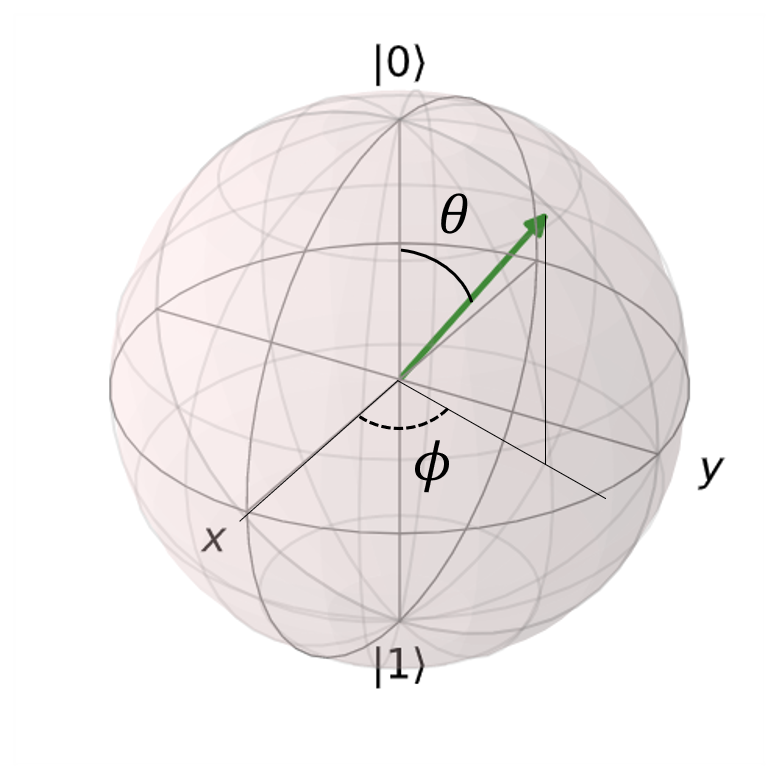
\includegraphics[width=5cm]{bloch.png}
                \caption{ブロッホ球}
            \end{center}
        \end{figure}
        $\ket{0}$を北極,$\ket{1}$を南極とした球を考えると、(2.3)は球面上のベクトルとして図示できる。
        このとき、$\theta$は状態ベクトルがz軸となす角、$\phi$はxy平面上に射影した状態ベクトルがx軸となす角とみなせる。
        状態ベクトルがx軸正方向に向くとき、$\ket{\psi} = \frac{(\ket{0}+\ket{1})}{\sqrt2}$であり、状態$\ket{0}$と$\ket{1}$が等確率で重ねあわされており($\ket{+}$状態)、y軸正方向を向くときには先ほどの重ね合わせ状態からz軸周りの位相が$\frac{\pi}{2}$変化した状態となる。($\ket{-}$状態)
        $\ket{0}$状態と$\ket{1}$状態の重ね合わせで表される純粋状態はすべてBloch球上の単位ベクトルとして表すことができる。

        \subsubsection{状態・期待値の測定}
        量子ビットの典型的な測定は{$\ket{0},\ket{1}$}による基底測定\footnote{測定に際して選ぶ基底は完全性を有する正規直交基底であれば何でもよいので,例として$\ket{+}$状態と$\ket{-}$状態の組み合わせを選ぶこともできる。}であり、測定により得られる状態は必ず0か1にランダムに収束する。
        状態が$\ket{\psi}$のとき、測定値i=0,1を得る確率は
        \begin{equation}
            P=|\inner<\psi,i>|^2
        \end{equation}
        で与えられる。このとき、先のブロッホ球における$\phi$、すなわち状態の位相の情報は失われる。このためブロッホ球上の$\phi$のみが異なる状態は測定によりすべて同じ状態として扱われる。\\
        また我々は量子ビットの状態だけでなく、準備した量子状態によって特定の物理量の期待値を測定するときがある。
        量子系における物理量はエルミート演算子$A$によって与えられ、状態$\ket{\psi}$のもとでの$A$の期待値$\langle A \rangle$は量子力学の公式より
        \begin{equation}
            \langle A \rangle =\langle \psi\ket{A\psi}
        \end{equation}
        で与えられる。

        \subsubsection{密度演算子}
        環境系との結合や複数の量子ビットが存在する状況下での1量子ビット状態には、混合状態という状態が存在する。
        例えば量子ビット$\ket{0}$,$\ket{1}$をそれぞれ1つずつ用意して箱に入れ、1つを取り出す場合、$\ket{0}$を取り出す確率、$\ket{1}$を取り出す確率はそれぞれ50\%である。
        しかしこの場合、取り出す1量子ビットの状態を重ね合わせを用いて$\ket{\psi} = \frac{(\ket{0}+\ket{1})}{\sqrt2}=\ket{+}$と書くことはできない。
        系全体で見たときに0,1の割合が50:50であることは既知であるが、1量子ビットについては0,1である確率がどのような割合で重ねあわされているか分からないためである。
        実際、状態$\ket{+}$は基底$\ket{+}$による測定で確率1を与えるが、上述の状態は必ず0か1かのどちらかであり、$\ket{+}$による測定でどちらの場合も確率1/2を与えるはずである。
        このような重ね合わせとは異なる、確率的に状態が与えられる状態を混合状態という。\\
        この混合状態を含めて量子ビットの状態を記述するために密度演算子というものを導入する。\\
        状態$\psi$のとりうる基底状態が$\{\ket{\psi_i}\}_{i=0}^N$であり、確率$p_i$で状態$\ket{\psi_i}$をとるとすると、その密度演算子$\rho$は
        \begin{equation}
            \rho_\psi=\sum_i^N p_i \ket{\psi_i}\bra{\psi_i}
        \end{equation}
        で与えられる。
        基底$\ket{\phi_0}$による状態$\rho_\psi$の測定結果は
        \begin{equation*}
            \bra{\phi_0}\rho_\psi\ket{\phi_0}
        \end{equation*}
        となる。また、物理量Aを状態$\rho$で測定した期待値は
        \begin{equation}
            \langle A \rangle =\mathrm{Tr}(\rho A)=\mathrm{Tr}(A\rho)
        \end{equation}
        で与えられる。\\
        先ほど例にあげた状態を密度演算子で記述すると、$p_0=1/2$, $p_1=1/2$より
        \begin{equation*}
            \rho=\frac{1}{2}\ket{0}\bra{0}+\frac{1}{2}\ket{1}\bra{1}
            =\left(
                \begin{array}{cc}
                  1/2 & 0\\
                  0 & 1/2\\
                \end{array}
              \right)
        \end{equation*}
        となり、$\bra{0}\rho\ket{0}=1/2$, $\bra{1}\rho\ket{1}=1/2$,さらに$\bra{+}\rho\ket{+}=1/2$であることから系の状態を正しく記述できている。
        重ね合わせ状態の密度演算子による表現は
        \begin{equation*}
            \rho=1\cdot\ket{+}\bra{+}
            =\left(
                \begin{array}{c}
                  1/\sqrt2\\
                  1/\sqrt2
                \end{array}
              \right)
              \left(
                \begin{array}{cc}
                  1/\sqrt2 & 1/\sqrt2  
                \end{array}
              \right)
            =\left(
                \begin{array}{cc}
                  1/2 & 1/2\\
                  1/2 & 1/2\\
                \end{array}
              \right)
        \end{equation*}
        となり、両者が明確に異なる状態であることがわかる。\\
        密度演算子は、いかなる状態の測定を行っても確率は0以上でありその総和は1という要請から
        \begin{eqnarray}
            \rho \geq 0 \\
            \mathrm{Tr}(\rho)=1
        \end{eqnarray}
        という性質を持つ。純粋状態に加え、単位ベクトルでは記述できない混合状態を表せる密度演算子は\\
        量子状態の最も一般的な表現を与える演算子である。

        \subsubsection{多量子ビット系の表現}
        ここでは2つ以上の量子ビットが存在する系(合成系)の表現について説明する。\\
        2つの量子ビットが存在しそれぞれの量子系にヒルベルト空間$\mathcal{H}_1,\mathcal{H}_2$が付随する場合、2量子ビット合成系に付随するヒルベルト空間$\mathcal{H}$は
        \begin{equation}
            \mathcal{H}=\mathcal{H}_1\otimes\mathcal{H}_2
        \end{equation}
        n量子ビット系なら
        \begin{equation}
            \mathcal{H}=\mathcal{H}_1\otimes\mathcal{H}_2\otimes\cdots\otimes\mathcal{H}_n
        \end{equation}
        に拡張される。ここで$\otimes$はテンソル積を表す。2量子ビット系の基底は互いの{$\ket{0},\ket{1}$}基底から1つずつを選んだ組み合わせのテンソル積を羅列し
        \begin{equation*}
            \ket{00}
            =\left(
                \begin{array}{c}
                    1 \\
                    0 \\
                    0 \\
                    0
                \end{array}
             \right),
            \ket{01}=\left(
                \begin{array}{c}
                    0 \\
                    1 \\
                    0 \\
                    0
                \end{array}
              \right),
            \ket{10}=\left(
                \begin{array}{c}
                    0 \\
                    0 \\
                    1 \\
                    0
                \end{array}
              \right),
            \ket{11}=\left(
                \begin{array}{c}
                    0 \\
                    0 \\
                    0 \\
                    1
                \end{array}
              \right)
        \end{equation*}
        となる。($\ket{\psi}\otimes\ket{\phi}$を$\ket{\psi\phi}$と略記する)\\
        状態については、互いの量子ビット間に後述する量子エンタングルメントがない場合、密度演算子$\rho_1,\rho_2$のテンソル積が合成系の状態
        \begin{equation}
        \begin{split}
            \rho &= \rho_1\otimes\rho_2\\
            \mathrm{両者が純粋状態} \ket{\psi_1},\ket{\psi_2} &\mathrm{の場合は} \ket{\psi}=\ket{\psi_1}\otimes\ket{\psi_2}
        \end{split}
        \end{equation}
        を与える。\\
        状態の確率および物理量の期待値は1qubitのときと同様、式(),()により得られる。\\
        量子ビット合成系を考えるとき重要になるのが、量子エンタングルメント(量子もつれ)という現象である。
        例として、以下のような2量子ビット系の状態ベクトル
        \begin{equation}
            \ket{\phi}=\frac{\ket{00}+\ket{11}}{\sqrt2}
        \end{equation}
        について考える。この状態は2量子ビット系の基底$\ket{00},\ket{11}$が等確率で重ねあわされた純粋状態であるが、
        ()もしくは()のように1量子ビット系の単位ベクトルまたは密度演算子どうしのテンソル積の形に分解することができない。\\
        いま、量子ビット1と2のそれぞれに対し、この状態が$\ket{0}$なのか$\ket{1}$なのかの測定を行うとする。
        量子ビット1の測定結果が$\ket{0}$であったとすると、$\ket{\phi}$は$\ket{00}$に収束するので、量子ビット2の測定結果も必ず$\ket{0}$になる。
        同様に、量子ビット1の測定結果が$\ket{1}$であったとすると、量子ビット2の測定結果も必ず$\ket{1}$になる。
        量子ビット1と2がどれだけ離れていようとも、互いのビットの測定結果は常に同じになる。
        さらにこの関係は、量子ビット1と2の観測者が同じ基底で測定を行う限り成立する。(計算は記さないが、例えば測定の基底を$\ket{+},\ket{-}$として
        ()の状態が$\ket{+}$か、$\ket{-}$かの測定を行った結果も量子ビット1,2両方で同じとなる。)
        このような古典系では考えられない強い相関は量子相関とよばれ、()のような状態(エンタングル状態)のもつ大きな特徴である。
        後述する2量子ビットゲートの目的はエンタングル状態を作り出すことにあり、この状態は量子計算アルゴリズムや量子テレポーテーションにおいて大きな有用性がある。
    
    \subsection{量子ビットの時間発展}
        \subsubsection{時間発展演算子}
        量子系のHamiltonianが$\hat{H(t)}$で表され、状態の波動関数が$\ket{\psi(t)}$である場合、
        Schr\"{o}dinger方程式により系の時間発展は
        \begin{equation}
            \frac{\partial}{\partial t}\ket{\psi(t)} = \hat{H(t)}\ket{\psi(t)}
        \end{equation}
        と表される。
        $\hat{H}$が時間に依存しないとしてこれを解くと、
        \begin{eqnarray}
            \ket{\psi(t)} = \exp (-\frac{i}{\hbar}\hat{H}t)\ket{\psi(0)}
        \end{eqnarray}
        という解が得られる。このとき$\ket{\psi(t)}$は$\ket{\psi(0)}$を
        \begin{eqnarray}
            U = \exp (-\frac{i}{\hbar}\hat{H}t)
        \end{eqnarray}
        という演算子によって変換した形になっていることがわかる。
        この演算子を時間発展演算子という。Hamiltonianはエルミート演算子であるため$U$のエルミート共役は
        \begin{eqnarray}
            U^\dagger = \exp (\frac{i}{\hbar}\hat{H}t)
        \end{eqnarray}
        となり、$U$の逆行列となる。自身のエルミート行列が逆行列となる演算子をユニタリ演算子といい、一般的な量子系の時間発展はユニタリ行列により与えられる。
        ユニタリ行列のベクトルへの作用を強調する場合は単に変換ともいう。

        \subsubsection{Pauli行列}
        量子ビットに対し行われる変換及び、量子ビットを記述するハミルトニアン(次節で後述)の中に頻繁に表れる演算子であるPauli行列について説明する。
        単位行列$I$およびPauli行列$\sigma_x,\sigma_y,\sigma_z$は以下の形で表される。
        \begin{equation}
            I=\left(
                \begin{array}{cc}
                    1 & 0 \\
                    0 & 1 \\
                \end{array}
              \right),
            \sigma_x=
              \left(
                \begin{array}{cc}
                    0 & 1 \\
                    1 & 0 \\
                \end{array}
              \right),
            \sigma_y=
              \left(
                \begin{array}{cc}
                    0 & -i \\
                    i & 0 \\
                \end{array}
              \right),
            \sigma_z=\left(
                \begin{array}{cc}
                    1 & 0 \\
                    0 & -1 \\
                \end{array}
              \right)
        \end{equation}
        $\sigma_x$は$\sigma_x \ket{0}=\ket{1}, \sigma_x \ket{1}=\ket{0}$を与えることからビット反転(bit flip)の操作を行っており、
        $\sigma_z$は$\sigma_z (\alpha\ket{0}+\beta\ket{1})=\alpha\ket{0}-\beta\ket{1}$を与えることから位相回転ゲート(phase flip)の操作を行う。\\
        ブロッホ球上のベクトルにPauli行列が作用した際どのような状態変化を起こすかを図()に示す。
        単位行列Iの作用は量子ビットの状態が変化しないことを表す。
        なお、1量子ビットについて$\sigma_x,\sigma_y,\sigma_z$の期待値の測定を行うことで状態密度$\rho$を
        \begin{equation}
        \begin{split}
            \rho  = \frac{1}{2}(I &+ \sum_{i=x,y,z} b_i \sigma_i)\\
            (b_i :\mathrm{Pauli演算子}\:\sigma_i&(i=x,y,z)\mathrm{の期待値})
        \end{split}
        \end{equation}
        のように求めることができる。
        (Blochベクトルを、1量子ビット状態のPauli行列の期待値を成分にもつベクトルとして定義することもできる)

    \section{超伝導素子による量子ビットの実装}
    この節では、先述した量子ビット系をどのように超伝導体素子を用いて実装したかについて説明する。
    超伝導量子ビットは超伝導体特有の非線形性を持たせた調和振動子によって構成される。
        \subsection{調和振動子系のハミルトニアン}
        最初に最も簡単な調和振動子について説明する。解析力学における一般的な調和振動子のハミルトニアンは$p,q$を一般化運動量、一般化座標を表す正準変数として
        \begin{equation}
            \mathcal{H}=\frac{1}{2m}p^2+\frac{1}{2}m\omega^2 q^2
        \end{equation}
        \begin{equation*}
            m:\mathrm{質量},\omega:\mathrm{固有周波数}
        \end{equation*}
        と記述される。このHamiltonianを量子化するために正準変数q,pを交換関係
        \begin{equation}
            [\hat{q},\hat{p}]=i\hbar
        \end{equation}
        をもつ演算子$\hat{q},\hat{p}$に置き換える。昇降演算子(生成消滅演算子)$\hat{a},\hat{a}^\dagger$を
        \begin{eqnarray}
            \hat{a}=\sqrt{\frac{m\omega}{2\hbar}}(\hat{q}+\frac{i}{m\omega}\hat{p})\\
            \hat{a}^\dagger=\sqrt{\frac{m\omega}{2\hbar}}(\hat{q}-\frac{i}{m\omega}\hat{p})
        \end{eqnarray}
        のように導入すると$\hat{a},\hat{a}^\dagger$間には
        \begin{equation}
        \begin{split}
            [\hat{a},\hat{a}^\dagger]&=\frac{m\omega}{2\hbar}([\hat{q},\hat{q}]-\frac{i}{m\omega}[\hat{q},\hat{p}]+\frac{i}{m\omega}[\hat{p},\hat{q}]+\frac{1}{m\omega^2}[\hat{p},\hat{p}])\\
            &=-\frac{i}{\hbar}[\hat{q},\hat{p}]\\
            &=1
        \end{split}
        \end{equation}
        という関係があり、これを用いると$\hat{q},\hat{p}$は
        \begin{eqnarray}
            \hat{q}&=&\sqrt{\frac{\hbar}{2m\omega}}(\hat{a}+\hat{a}^\dagger)\\
            \hat{p}&=&-i\sqrt{\frac{\hbar}{2}m\omega}(\hat{a}+\hat{a}^\dagger)
        \end{eqnarray}
        と書ける。これをもとに先ほどのHamiltonianは
        \begin{equation}
        \begin{split}
            \mathcal{H}&=\frac{\hbar\omega}{4}(\hat{a}+\hat{a}^\dagger)^2-\frac{\hbar\omega}{4}(\hat{a}-\hat{a}^\dagger)^2\\
            &=\frac{\hbar\omega}{2}(\hat{a}\hat{a}^\dagger+\hat{a}^\dagger\hat{a})\\
            &=\hbar\omega(\hat{a}^\dagger\hat{a}+\frac{1}{2})\\
        \end{split}
        \end{equation}
        と記述される。さらに定数項の部分をエネルギーの基準点に対応させ無視することで最終的には
        \begin{equation}
            \mathcal{H}=\hbar\omega\hat{a}^\dagger\hat{a}
        \end{equation}
        と書くことができる。
        \subsubsection{LC共振器}
        先ほどの調和振動子系は、工学的にはLC共振器の形で実装される。
        図()のようなLC共振器について考える。
        \begin{figure}
            \begin{center}
                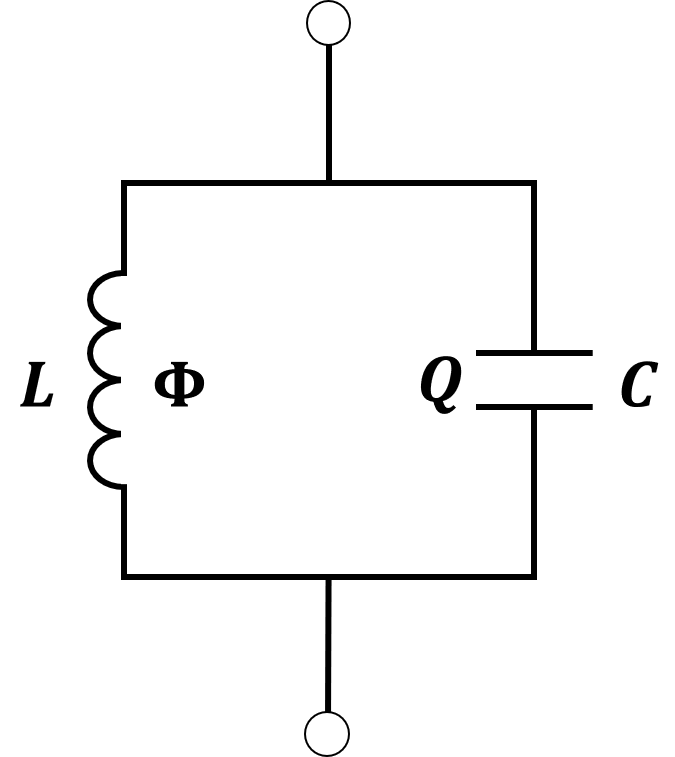
\includegraphics[width=4cm]{LCResonator.png}
                \caption{LC共振器}
            \end{center}
        \end{figure}
        一般化座標として磁束$\Phi$を用いることとすると、Faradayの法則及びインダクタンス$L$の定義式から
        \begin{eqnarray}
            V&=&\frac{d\Phi}{dt}=\dot{\Phi},\\
            \Phi&=&-LI
        \end{eqnarray}
        が導かれる。回路の運動エネルギー$T$及びポテンシャルエネルギー$U$は、
        \begin{eqnarray}
            T=C\int V dV & = & \frac{1}{2}C \dot{\Phi}^2,\\
            U=L\int I dI & = & \frac{1}{2L} \Phi^2
        \end{eqnarray}
        で与えられ、これよりLagrangian\quad$\mathcal{L}$は
        \begin{equation}
            \mathcal{L}(\Phi,\dot{\Phi})=T-U=\frac{1}{2}C \dot{\Phi}^2-\frac{1}{2L} \Phi^2
        \end{equation}
        と記述される。したがって一般化運動量$Q$は
        \begin{equation}
            Q = \frac{\partial\mathcal{L}}{\partial \dot{\Phi}}=C\dot{\Phi}
        \end{equation}
        となる。HamiltonianはLagrangianをLegendre変換して
        \begin{equation}
            \mathcal{H}(\Phi,Q)=Q\dot{\Phi}-\mathcal{L}=\frac{1}{2C}Q^2+\frac{1}{2L}\Phi^2
        \end{equation}
        と求まる。
        ()式は()式において
        \begin{equation}
        \begin{split}
             q \to Q,\; &p \to -\Phi,\\
             m\omega^2 \to \frac{1}{C},\; m \to &L, \; \omega \to \frac{1}{\sqrt{LC}}
        \end{split}
        \end{equation}
        と置き換えたものと等価であり、調和振動子の場合と同様にこの系も量子化が可能である。正準変数$\hat{Q},\hat{\Phi}$と昇降演算子$\hat{a},\hat{a}^\dagger$は
        \begin{eqnarray}
            \hat{Q}=\sqrt{\frac{\hbar}{2}\omega C}(\hat{a}+\hat{a}^\dagger)\\
            \hat{\Phi}=i\sqrt{\frac{\hbar}{2}\frac{1}{\omega C}}(\hat{a}-\hat{a}^\dagger)
        \end{eqnarray}
        という関係式で結ばれ、最終的には定数項を落とすことでHamiltonianを()式同様
        \begin{equation}
            \mathcal{H}=\hbar\omega\hat{a}^\dagger\hat{a}
        \end{equation}
        の形に書くことができる。
        \subsection{ジョセフソン接合}
        2つの超伝導体の間に絶縁体もしくは常伝導体などの極めて薄い障壁をさしはさむことにより、2つの超伝導体間には超伝導電流が流れる。
        1962年にB. D. Josephsonによって発見されたこの効果をジョセフソン効果、超伝導体-障壁-超伝導体の接合をジョセフソン接合という。\\

        \begin{figure}[H]
            \begin{center}
                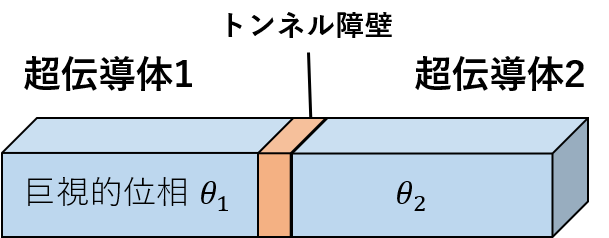
\includegraphics[width=7cm]{JJ.png}
                \caption{ジョセフソン接合}
            \end{center}
        \end{figure}

        金属が超伝導体となるとき、すべての電子が同じふるまいをする巨視的量子状態が出現し、電子の波動関数は粒子数$N$と巨視的位相$\theta$によって記述される。
        超伝導体1,2の巨視的位相をそれぞれ$\theta_1,\theta_2$とすると、流れる電流$I$は位相差$\varphi=\theta_1-\theta_2$を用いて
        \begin{equation}
            I=I_c \sin\varphi
        \end{equation}
        という式で表される(直流ジョセフソン効果)。ここで、$I_c$はジョセフソン接合を流れる最大の電流であり、臨界電流と呼ばれる。
        $I_c$はAmbegaokar=Baratoffの式より以下のように求められ
        \begin{equation}
            I_c=\frac{\pi \Delta(T)}{2eR_n}\tanh(\frac{\Delta(T)}{2k_BT})
        \end{equation}
        \begin{equation*}
            T:\mathrm{絶対温度},\quad \Delta(T):超伝導体のバンドギャップ,\quad R_n:障壁の抵抗
        \end{equation*}
        温度依存性を有するが、実験での量子ビット系は$T \sim 10$mKの温度領域におかれるため上式は
        \begin{equation}
            I_c=\frac{\pi \Delta(0)}{2eR_n}
        \end{equation}
        と近似できる。式(),()から分かるように、流れる臨界電流は超伝導体間の電位差に関係なく、位相差のみによって決定される。\\
        ジョセフソン接合における電位Vと位相差$\varphi$の間には以下の関係があり、
        \begin{equation}
            \frac{\partial\varphi}{\partial t}=\frac{2e}{\hbar}V
        \end{equation}
        で表せることが知られている(交流ジョセフソン効果)。()式、()式を用いると、ジョセフソン接合が持つポテンシャルエネルギーは
        \begin{equation}
        \begin{split}
            U&=\int IVdt \\
            &= \frac{\hbar I_c}{2e}\int \sin \varphi \frac{d\varphi}{dt}dt \\
            &= -E_J \cos \varphi
        \end{split}
        \end{equation}
        となり、非線形な項で表されることになる。ここで、
        \begin{equation}
            E_J=\frac{\hbar I_c}{2e}
        \end{equation}
        はジョセフソンエネルギーと呼ばれる量である。\\
        ジョセフソン接合の回路記号を以下図()のように表す。なお実際のジョセフソン接合には()式中の障壁の抵抗$R_n$の他にキャパシタンス$C_J$が存在し、
        図()のように接合に並列に含まれていると考える。
        \begin{figure}[htbp]
            \begin{center}
                \begin{tabular}{c}
                    \begin{minipage}{0.5\hsize}
                        \begin{center}
                            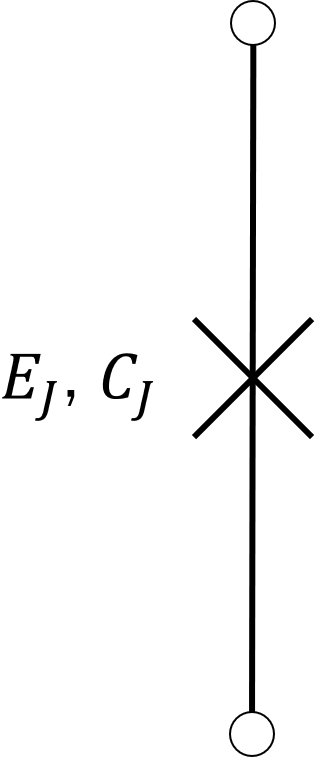
\includegraphics[width=1.5cm]{Joseph.png}
                        \end{center}
                        \captionsetup{labelformat=empty,labelsep=none}
                        \caption{[a]}
                    \end{minipage}
                    
                    \begin{minipage}{0.5\hsize}
                        \begin{center}
                            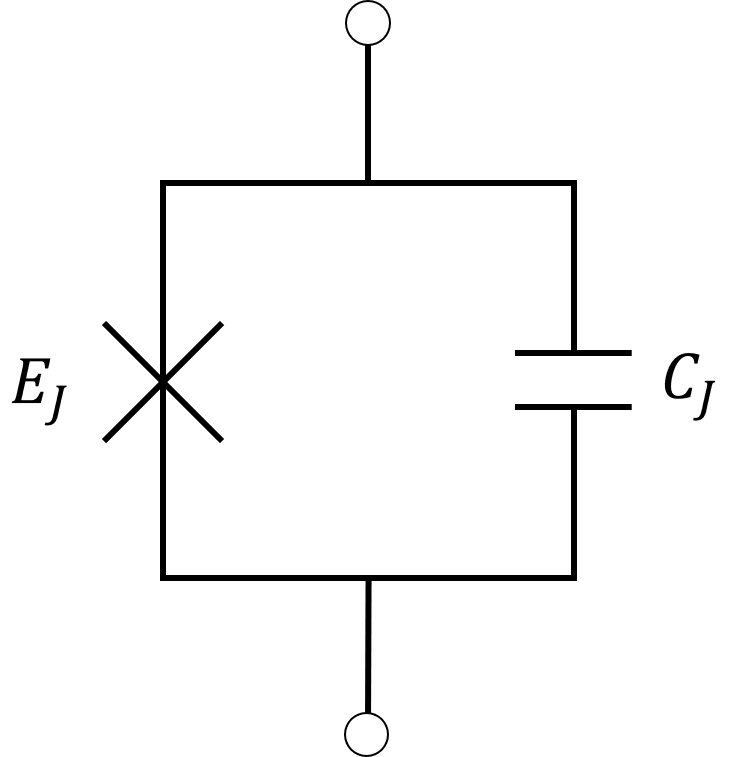
\includegraphics[width=3cm]{Joseph_real.png}
                        \end{center}
                        \captionsetup{labelformat=empty,labelsep=none}
                        \caption{[b]}
                    \end{minipage}
                \end{tabular}
                \caption{ジョセフソン接合の回路記号}
            \end{center}
        \end{figure}
        \subsubsection{DC-SQUID}
        次に、ジョセフソン接合を利用した素子であるSQUID(Superconducting quantum interference device) について説明する。
        DC-SQUIDは図()のような、ジョセフソン接合が2つ挿入された超伝導体ループから形成される。
        \begin{figure}
            \begin{center}
                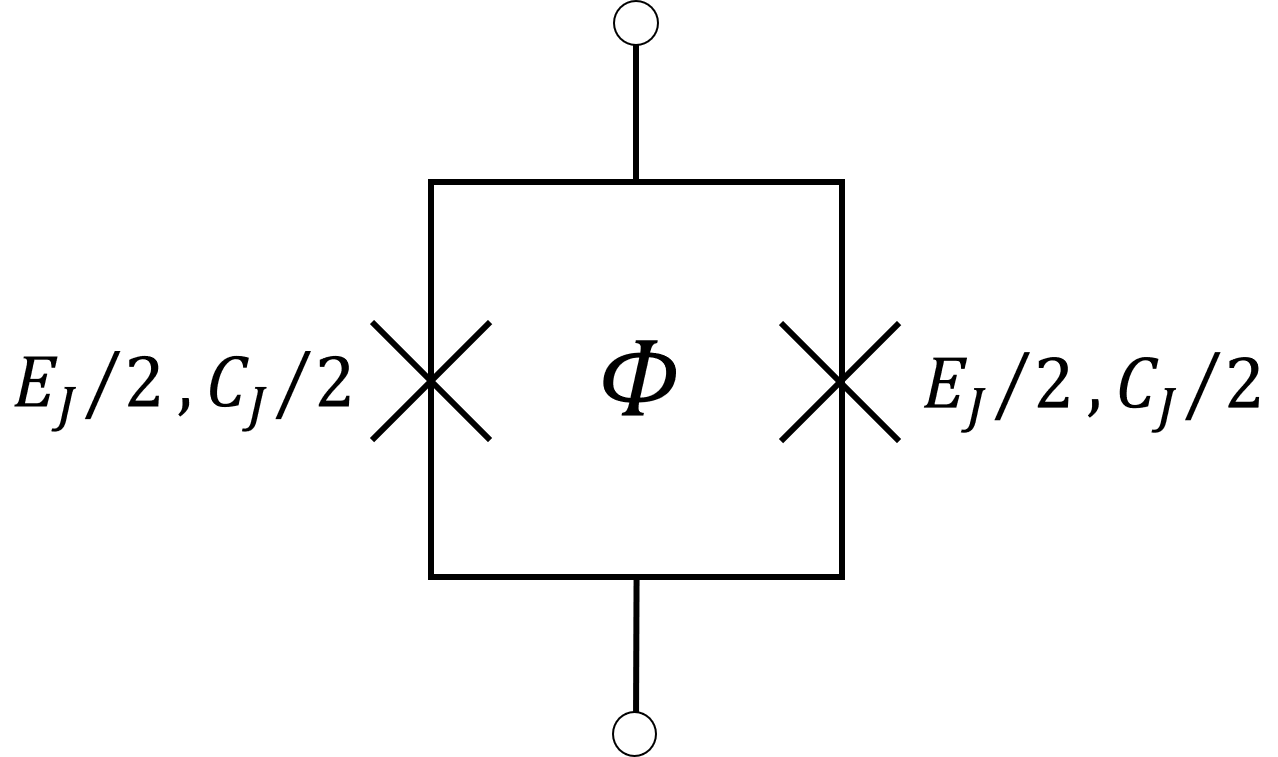
\includegraphics[width=5cm]{DCsquid.png}
                \caption{DC-SQUID}
            \end{center}
        \end{figure}
        Josephson接合のときと同様、ポテンシャルエネルギーを計算すると
        \begin{equation}
        \begin{split}
             U&=-\frac{E_J}{2} \cos \varphi_1-\frac{E_J}{2} \cos \varphi_2\\
            &=-E_J \cos (\frac{\varphi_1+\varphi_2}{2})\cos (\frac{\varphi_1-\varphi_2}{2})
        \end{split} 
        \end{equation}
        となる。ここで、超伝導ループにおける磁束の量子化の条件より
        \begin{equation}
        \begin{split}
            \frac{2\pi \Phi}{\Phi_0}+\varphi_1-\varphi_2=0 , \;  \Phi_0 = 2\pi\frac{\hbar}{2e}\\
            \Phi_0 : \mathrm{磁束量子(flux quanta)}
        \end{split}    
        \end{equation}
        を利用し、()式は
        \begin{equation}
            U=-E_J \cos (\frac{\varphi_1+\varphi_2}{2})\cos (\pi\frac{\Phi}{\Phi_0})
        \end{equation}
        と書き換えられる。()式と比較すると、
        \begin{equation}
            E_J \to E_J \cos (\pi\frac{\Phi}{\Phi_0}) , \;\varphi \to \frac{\varphi_1+\varphi_2}{2}
        \end{equation}
        という対応関係があることが分かる。これによってSQUIDは外部からの磁束$\Phi$によってジョセフソンエネルギーを変化させられる
        ジョセフソン接合として扱うことができる。
        \subsection{SQUIDによる量子ビットの実装}
        ジョセフソン接合によりポテンシャルエネルギーに非線形性を持たせ、なおかつSQUIDの導入によりそれを外部磁束で制御できるようになることを示した。
        ここからはLC共振器とSQUIDによって量子ビットを実装する方法について説明する。
        図()のようにキャパシタンス$C_g$を介してジョセフソン接合に電圧$V_g$がかかっている系を考える。
        \begin{figure}[H]
            \begin{center}
                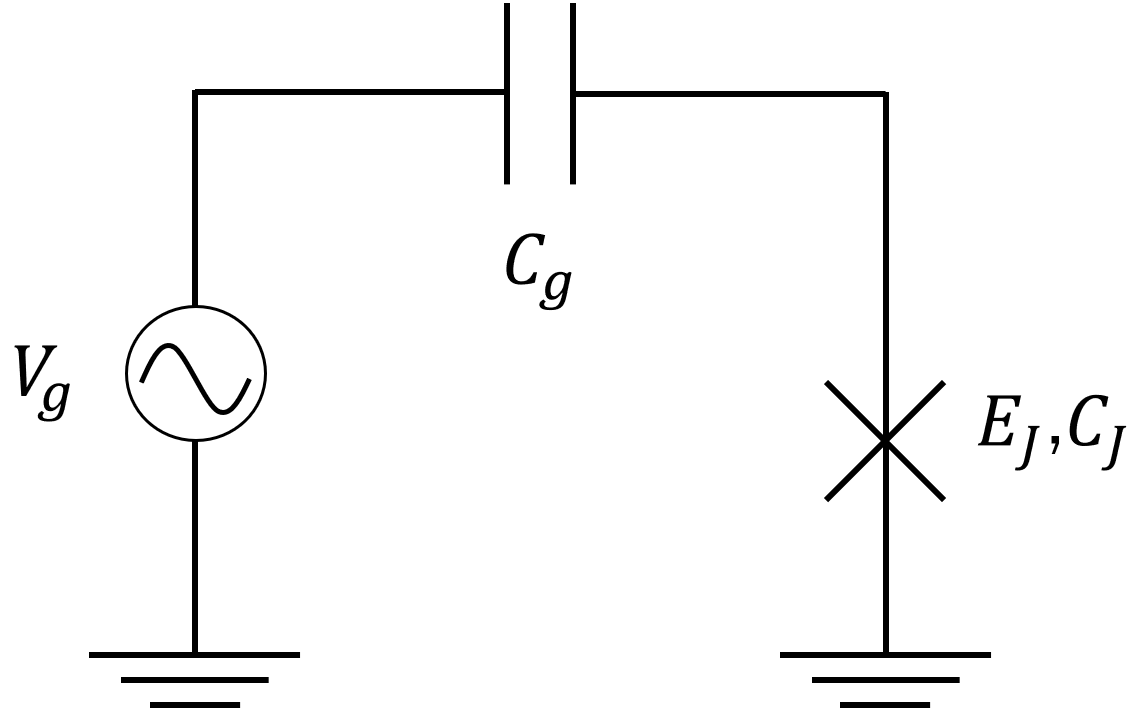
\includegraphics[width=5cm]{CPB.png}
                \caption{クーパー対箱}
            \end{center}
        \end{figure}
        運動エネルギーT,ポテンシャルエネルギーUは磁束$\Phi$を一般化座標として
        \begin{eqnarray}
            T=\frac{1}{2}C_J\dot{\Phi}^2+\frac{1}{2}C_g(\dot{\Phi}-V_g)^2\\
            U=-E_J\cos(\phi)
        \end{eqnarray}
        となる。ここでジョセフソン接合における位相差$\phi$はジョセフソン効果の式から磁束$\Phi$と
        \begin{equation}
            \dot{\Phi}=\frac{\hbar}{2e}\dot{\phi}
        \end{equation}
        という関係を持つ。
        一般化座標を$\phi$におきかえるとLagrangianは
        \begin{equation}
            \frac{1}{2}\left(\frac{\hbar}{2 e}\right)^{2} C_{J} \dot{\phi}^{2}+\frac{1}{2} C_{g}\left(\frac{\hbar}{2 e} \dot{\phi}-V_{g}\right)^{2}+E_{J} \cos \phi
        \end{equation}
        となり、位相差$\phi$に共役な変数$q$は
        \begin{equation}
            q=\frac{\partial \mathcal{L}}{\partial \dot{\phi}}=\left(\frac{\hbar}{2 e}\right)^{2} C_{J} \dot{\phi}+\frac{\hbar}{2 e} C_{g}\left(\frac{\hbar}{2 e} \dot{\phi}-V_{g}\right)=\frac{\hbar}{2 e} Q
        \end{equation}
        という関係にある。以上よりLegendre変換を用いてHamiltonianは
        \begin{equation}
        \begin{split}
            \mathcal{H}(\phi, q)
            &=q \dot{\phi}-\mathcal{L}\\
            &=\frac{1}{2}\left(\frac{\hbar}{2 e}\right)C_{J} \dot{\phi}^{2}+\frac{1}{2}\left(\frac{\hbar}{2 e}\right)^{2} C_{g} \dot{\phi}^{2}-\frac{1}{2} C_{g} V_{g}^{2}-E_{J} \cos \phi
        \end{split}
        \end{equation}
        と求められる。\\
        超伝導体内における電荷は、2つの電子が電子-格子相互作用によって対をなしたCooper対と呼ばれるものであり
        超伝導体の電荷数$n$を
        \begin{equation}n=\frac{Q}{2 e}=\frac{q}{\hbar}\end{equation}
        と定める。またゲート電圧$V_g$が掛かっている部分の電荷数について
        \begin{equation}n_{g}=-\frac{C_{g} V_{g}}{2 e}\end{equation}
        と定めれば
        \begin{equation}\mathcal{H}(\phi, q)=\frac{(2 e)^{2}}{2\left(C_{J}+C_{g}\right)}\left(n-n_{g}\right)^{2}-\frac{(2 e)^{2}}{2 C_{g}} n_g^{2}-E_{J} \cos \phi\end{equation}
        と書ける。ここで量子ビットの帯電エネルギー、すなわちジョセフソン帯電エネルギーを
        \begin{equation}E_{C}=\frac{e^{2}}{2 C_{\Sigma}}, \quad C_{\Sigma}=C_{J}+C_{g}\end{equation}
        で定義する。以上により定数項を落としたハミルトニアンは
        \begin{equation}\mathcal{H}=4 E_{C}\left(n-n_{g}\right)^{2}-E_{J} \cos \phi\end{equation}
        のように記述される。\\
        このHamiltonianの量子化のため、正準変数$\phi,q$に対し交換関係
        \begin{equation}[\hat{\phi}, \hat{q}]=i \hbar\end{equation}
        を導入する。ここで$\hat{n}=\hat{q} / \hbar$であるため
        \begin{equation}[\hat{\phi}, \hat{n}]=\frac{1}{\hbar}[\hat{\phi}, \hat{q}]=i\end{equation}
        が成立する。電荷数$\hat{n}$はエルミート演算子であるため固有状態$\ket{n}$と固有値$n$を用いて
        \begin{equation}\hat{n}=\sum_{n} n|n\rangle\langle n|\end{equation}
        と書くことができる。
        このとき$e^{\pm i \hat{\phi}}$は昇降演算子となることが知られており
        \begin{equation}e^{i \hat{\phi}}=\sum_{n}\ket{n+1}\bra{n}, \quad e^{-i \hat{\phi}}=\sum_{n}\ket{n}\bra{n+1}\end{equation}
        と書ける。これにより
        \begin{equation}
            \cos \hat{\phi} = \frac{1}{2}(e^{i \hat{\phi}}+e^{-i \hat{\phi}})=\frac{1}{2}\sum_{n}(\ket{n+1}\bra{n}+\ket{n}\bra{n+1})
        \end{equation}
        となるので電荷量子ビットのHamiltonianは
        \begin{equation}\begin{aligned}
            \hat{\mathcal{H}} &=4 E_{C}\left(\hat{n}-n_{g}\right)^{2}-E_{J} \cos \hat{\phi} \\
            &=4 E_{C} \sum_{n}\left(n-n_{g}\right)^{2}\ket{n}\bra{n}-\frac{E_{J}}{2} \sum_{n}(\ket{n+1}\bra{n}+\ket{n}\bra{n+1})
            \end{aligned}\end{equation}
        となる。
    \subsection{他素子との結合}
        \subsubsection{共振器との結合}
        \subsubsection{量子ビットとの結合}
    \subsection{デコヒーレンス}
        \subsubsection{$T_1$,$T_2$,$T_2^E$}

\section{量子ビットゲート}
    \subsection{1qubitゲート}
        \subsubsection{X,Y軸回転}
        \subsubsection{Z軸回転}
        \subsubsection{その他の重要1qubitゲート}
    \subsection{CZゲート}
        \subsubsection{CZゲートの理論}
        \subsubsection{実装上の課題1.CZゲートの断熱・非断熱過程}
        \subsubsection{実装上の課題2.低周波磁束ノイズ}
        \subsubsection{パルス制御}

        
        